% Compile twice with XeLaTeX from this directory. Korean: xeCJK + Noto Serif CJK KR.
\documentclass[11pt,a4paper]{article}
\usepackage[margin=22mm]{geometry}
\usepackage{fontspec,xeCJK}
\xeCJKsetup{CJKspace=true}
\setmainfont{Latin Modern Roman}
\setCJKmainfont{Noto Serif CJK KR}
\setCJKsansfont{Noto Sans CJK KR}
\setCJKmonofont{Noto Sans CJK KR}
\usepackage{amsmath,amssymb,mathtools,bm}
\usepackage{graphicx,booktabs,array,longtable,caption,float}
\usepackage[unicode,colorlinks=true,urlcolor=blue,linkcolor=blue]{hyperref}
\usepackage{xurl}
\usepackage{enumitem}
\setlist{nosep,leftmargin=*}
\setlength{\parskip}{5pt}
\setlength{\parindent}{0pt}
\setlength{\emergencystretch}{3em}
\newcommand{\ind}{\mathbf{1}}
\newcommand{\sg}{\operatorname{stopgrad}}
\newcommand{\med}{\operatorname{median}}
\newcommand{\mean}{\operatorname{mean}}
\newcommand{\diag}{\operatorname{diag}}
\newcommand{\dilate}{\operatorname{dilate}}
\newcommand{\erode}{\operatorname{erode}}
\newcommand{\RGB}{\mathrm{RGB}}
\newcommand{\calB}{\mathcal{B}}
\title{다중 시기 항공영상의 동적 차량 제거를 위한 텍스처 베이킹\\\large 쉬운 장면, 고점유 장면 및 개선 기준선의 통합 보고서}
\author{실험 기록 통합본}
\date{실험: 2026년 10월 25--26일 \quad 문서 작성: 2026년 10월 26일}
\begin{document}
\maketitle
\begin{abstract}
동일 위치의 다중 시기 사진을 하나의 텍스처로 베이킹할 때 차량 관측을 제외하는 가중치 $S$의 효과를 조사했다. Block-NeRF형 의미 마스크, NeRF-HuGS형 일관성 마스크, RobustNeRF형 잔차 가중치를 동일한 평면 베이킹에 적용했다. 빈 배경이 다수인 쉬운 장면에서는 미적용 L2와 시간 중앙값도 강한 결과를 보였으나, 차량이 다수 시기에 관측되는 두 장면에서는 잔차 선택의 실패와 관측 부족이 드러났다. 이에 UV 좌표에서 비차량 관측만 합성하고 미관측 영역을 공간 보간하는 기준선 및 마스크 투영ㆍ초기화ㆍ공간 정규화 변형을 비교했다. 그림자 후보 제외를 추가한 직접 UV 합성은 고점유 차량 위치 PSNR에서 B 21.00dB, C 22.23dB를 얻었으며, 기존 Block형 대비 각각 약1.06dB, 1.25dB 높았다. 결과는 실제 정사사진을 사용하는 반합성 평면 실험에 한정된다. 미관측 배경의 보간과 어두운 잔상이 남아 완전한 차량 제거를 뜻하지 않는다.
\end{abstract}
\tableofcontents
\clearpage
\section{Intro}
\subsection{문제와 연구 질문}
서로 다른 시기에 촬영한 영상 $I_i$를 한 장의 텍스처 $T$로 모으면 차량 색도 배경에 섞인다. 본 실험은 메쉬 $M$과 카메라 $\pi_i$를 고정하고 관측 가중치 $S_i$를 바꿨을 때, 차량 잔상 억제와 지면 디테일 보존이 어떻게 달라지는지를 묻는다. 학습 대상은 NeRF 방사장 전체가 아니라 지면 텍스처 및 시점별 색보정이다.

세 단계의 실험은 다음 논리로 연결된다.
\begin{enumerate}
\item \textbf{Easy:} 여러 해에 지면이 비고 특정 해에 차량이 많은 장면에서 공통 베이킹과 기존 $S$를 검증한다.
\item \textbf{Hard:} Easy에서 L2도 잘 나온 원인이 빈 관측의 다수 여부인지 확인하기 위해, 차량이 5회 중 3--4회 나타나는 두 실제 장면을 추가한다.
\item \textbf{Improved:} Hard에서의 실패를 바탕으로, 소수의 비차량 관측을 직접 합성하고 관측 부족에 공간 사전정보를 넣는 개선 기준선을 비교한다.
\end{enumerate}

\subsection{범위와 용어}
Block-NeRF, NeRF-HuGS, RobustNeRF는 관측 선택의 아이디어를 제공한다~\cite{block,hugs,robust}. 이하 ``형''이라는 표현은 본 실험의 베이킹용 구현을 가리키며 원 논문의 전체 NeRF 학습 재현을 뜻하지 않는다. 제거는 차량 메쉬를 삭제하는 것이 아니라 차량이 찍힌 영상의 색을 텍스처 학습에서 제외하는 것이다. 주차된 정지 차량도 의미 마스크에서는 제거 대상이다.

Easy 문서의 과거 ``차량 내부''는 자동차 실내가 아니다. 실제로는 차체 위치에 둔 반경5텍셀 원형 표본이었다. 본 보고서는 이를 \textbf{차량 위치 표본}으로 부르고, Hard에서는 차량 전체 OBB 영역 평가와 명확히 구분한다.

\section{Method}
\subsection{영상 출처, 장면과 전처리}
원본은 PDOK가 제공하는 Beeldmateriaal Nederland의 연도별 항공 정사영상이다. 서비스는
\url{https://service.pdok.nl/hwh/luchtfotorgb/wms/v1_0}이며, Google Maps 캡처나 논문 제공 장면을 사용하지 않았다. 출처 표기는 Beeldmateriaal Nederland / PDOK, CC BY 4.0이다. 제공처 안내는 참고자료에 기재했다. 영상은 다운로드 후 정합ㆍ색 정규화ㆍ투영ㆍ베이킹으로 가공했다.

WMS 1.3.0 GetMap으로 같은 장면의 같은 bbox를 요청하고 레이어를 \texttt{2021\_orthoHR}부터 \texttt{2026\_orthoHR}까지 바꿨다. 요청은 EPSG:4326, $1500\times1500$px, 약 $120\times120$m다. 약8cm/px는 요청 격자 간격으로 실제 촬영 해상도와 구별해야 한다. PNG를 요청했으나 기록된 응답의 실제 인코딩은 JPEG다. 연도는 레이어 이름이며 정확한 비행일은 확인하지 않았다.

\begin{table}[htbp]\centering\small
\caption{최종 사용한 실제 장면. 차량 점유는 검출 기반 대리 지표다.}\label{tab:data}
\begin{tabular}{lccp{57mm}}
\toprule 장면 & 중심 위도 & 중심 경도 & 학습 데이터 특성\\\midrule
Easy & 52.08235 & 5.10090 & Jaarbeurs 남쪽 주차장, 차량 관측 대부분1/5\\
Hard B & 52.07400 & 5.04600 & 차량 경험 픽셀 중3회 이상 점유68.1\%\\
Hard C & 52.07730 & 5.04895 & 차량 경험 픽셀 중3회 이상 점유63.0\%\\\bottomrule
\end{tabular}\end{table}

최초 Jaarbeurs 후보(52.08718, 5.10243)는 공사로 변해 제외했다. 최종 Easy의 학습 ROI 차량 검출 수는 2021--2025년에 $3,0,0,0,223$이었다. 그중 차량 검출 경험 픽셀의 99.1\%는 한 해만 점유했다. B의 학습 차량 마스크 면적은 약49--59\%, C는 약46--55\%였다.

Easy는 SIFT와 RANSAC 유사변환으로2023년 기준 정합을 수행했다. 반복 차량 패턴이 많은 Hard에서는 잘못된 전역 매칭을 피하기 위해 지리 좌표의 초기 정렬을 이용한 CLAHEㆍLK 전후방 추적과 제한된 변위, RANSAC 유사변환을 사용했다. Hard의 정합 inlier 중앙 오차는 B 약0.41--0.97px, C 약0.34--0.75px였지만 일부 연도의 inlier가 적어 전역 정확도를 보장하지 않는다. 지면의 강건한 채널별 gain/bias로 노출을 정규화했다. 모든 방법은 같은 전처리 결과를 사용한다.

학습은2021--2025년, 시간 hold-out은2026년이다. 2026은 전처리를 거치지만 텍스처 초기화ㆍ관측 선택 학습ㆍ최적화 손실에는 사용하지 않는다. Easy의 \texttt{2026\_quickorthoHR}는 별도로 받았으나 독립 촬영 여부가 불명확해 제외했다. 합성 사선 카메라4장은 동일 연도 사진의 재투영으로, 독립 촬영4회가 아니다.

\subsection{표기와 공통 베이킹 모델}
연도를 $t\in\{1,\ldots,5\}$, 합성 카메라를 $c\in\{0,1,2,3\}$, 입력 번호를 $i=(t,c)$로 둔다. $J_t(u)\in[0,1]^3$는 정합ㆍ노출 정규화된 정사영상의 UV 위치 $u$의 색이다. $\phi_c(r)$는 카메라 픽셀 $r$에서 지면 UV로 가는 homography다.
\begin{equation}
 I_{t,c}(r)=J_t(\phi_c(r)),\qquad T_\theta=U_{512\to1024}(\theta),\quad
 \theta\in[0,1]^{512\times512\times3}.
\end{equation}
$U$는 bilinear 보간이며 구현은 \texttt{align\_corners=True}를 사용한다. 평면 메쉬는 $x,y\in[-60,60]$m, $z=0$이다. 카메라는 원점을 바라보며 중심 거리100m, 초점거리480px, 출력 $768\times576$이다. 기울기/방위는 $(0,0),(20,0),(35,100),(45,220)$도다. 기울어진 카메라의 고도는 $100\cos(\text{기울기})$m이므로 거리와 고도를 혼동하면 안 된다.

학습 예측과 RGB 평균 제곱 오차는
\begin{align}
 P_i(r)&=A_i\,R(M,T_\theta;\pi_c)(r)+b_i
        =A_i\,T_\theta(\phi_c(r))+b_i,\\
 e_i(r)&=\frac{1}{3}\|P_i(r)-I_i(r)\|_2^2,\qquad
 \varepsilon_i(r)=\sqrt{e_i(r)}.
\end{align}
$A_i\in\mathbb R^{3\times3},b_i\in\mathbb R^3$는 시점별 색보정이다. $V_c(r)$는 평면 내부의 valid 마스크이며 차량 마스크 $S_i(r)$ 및 평가 ROI와 다르다. 정규화 텍스처 좌표의 최댓값이0.98이하인 곳만 valid로 둔다.

선택한 영상 batch $\calB$의 실제 목적함수는
\begin{align}
 \mathcal L_{\rm data}
 &=\frac{\sum_{i\in\calB}\sum_r V_c(r)S_i(r)e_i(r)}
         {\max(1,\sum_{i\in\calB}\sum_r V_c(r))},\label{eq:data}\\
 \mathcal L_{\rm color}
 &=10^{-3}\left[\mean_{i,a,b}(A_i-I_3)_{ab}^2+
                       \mean_{i,a}(b_i)_a^2\right],\\
 \mathcal L_{\rm bake}&=\mathcal L_{\rm data}+\mathcal L_{\rm color}.
\end{align}
분모는 $\sum VS$가 아니라 $\sum V$다. 따라서 $S$가 작아지면 데이터항의 규모도 감소하고, 동일한 정규화 계수의 상대 영향은 커질 수 있다. 이는 실제 구현의 공통 조건이지 유효 관측 수 보정이 아니다. $A_i=I_3,b_i=0$에서 시작하고2023년 nadir의 색보정을 고정해 색 좌표의 기준으로 삼는다.

\subsection{공통 최적화 절차}
기본 초기값은 $\theta^{(0)}=D_{1024\to512}(\frac15\sum_tJ_t)$이다. 매번20개 학습 영상 중4개를 뽑고, 렌더ㆍ색보정ㆍ마스크 생성ㆍ손실 계산ㆍ역전파ㆍAdam 갱신ㆍ$[0,1]$ clamp를 수행한다. 최적화는600회의 optimizer update이며600 epoch가 아니다. 텍스처 학습률은0.025, 색보정은0.001이다. Easy는seed42, Hard 주요4방법과 학습형 개선안은seed42/43/44를 사용했다. 메쉬, 카메라, 입력 영상은 최적화하지 않는다. 최종 텍스처는 특정 카메라의 색보정을 적용하지 않은 $T_\theta$다.

\subsection{미적용 기준선: L2와 시간 중앙값}
\paragraph{L2 / no-removal.}
모든 valid 관측을 쓰므로 $S_i(r)\equiv1$이다. L2 norm 자체는 $\|x\|_2=\sqrt{\sum_kx_k^2}$지만 여기서 L2 손실은 그 제곱의 RGB 평균, 즉 MSE다. 모델 이름이나 가중치 decay를 뜻하지 않는다. 색보정과 카메라 재표본화를 생략하고 한 texel만 보면
\begin{equation}
 \arg\min_z\sum_{t=1}^5\|z-J_t(u)\|_2^2
 =\frac15\sum_{t=1}^5J_t(u).
\end{equation}
따라서 빈 배경이 다수이면 차량이 희석되고 차량이 다수이면 그 색이 남는다. 이 평균식은 직관을 위한 단순화로 실제600회 베이킹이 정확한 시간 평균과 같다는 뜻은 아니다.

\paragraph{시간 중앙값.}
\begin{equation}
 T_{{\rm median},k}(u)=\med_{t=1,\ldots,5}J_{t,k}(u),\quad k\in\{R,G,B\}.
\end{equation}
이 채널별 중앙값은 $\sum_t|z-J_{t,k}(u)|$의 최소화 해다. 다수 오염에 약하며 RGB 채널별 선택값이 서로 다른 연도에서 올 수도 있다. 원래 중앙값 참고 기준선은1024격자의 사진에 직접 적용하고512기저 베이킹은 거치지 않았다. 뒤의 UV fusion은 공통512기저를 거친다.

\subsection{Block-NeRF형: 의미 클래스에 따른 관측 제외}
검출된 차량 OBB 집합을 $\mathcal O_i$라 하면
\begin{equation}
 D_i(r)=\ind\left[r\in\dilate_{5\times5}\left(\bigcup_{o\in\mathcal O_i}\operatorname{polygon}(o)\right)\right],
 \qquad S_i^{\rm Block}(r)=1-D_i(r).
\end{equation}
DOTA 사전학습 YOLO11s-OBB의 small/large vehicle(class9/10), confidence0.25, 최대1000개를 사용했다. 이 $S$는 고정한다. 원 Block-NeRF의 Panoptic-DeepLab을 항공영상용 OBB 검출기로 바꿨으며, 알려진 포즈를 사용하므로 COLMAP 마스킹은 생략했다. 차체 누락과 그림자는 남을 수 있고, 모든 시기에 가린 지면은 마스크만으로 알아낼 수 없다.

\subsection{NeRF-HuGS형: 특징점 지지, 잔차와 SAM 영역}
\paragraph{특징점 일관성.}
20개 영상의 모든 쌍에 SIFT ratio0.75와 homography RANSAC2px를 적용한다. 특징점 $j$가 검증된 매칭으로 지지받는 서로 다른 영상 수를 자기 자신을 포함해 $n_{ij}$로 두면
\begin{equation}
 q_{ij}=\ind[n_{ij}\ge5]=\ind[n_{ij}/20\ge0.25].
\end{equation}
$q_{ij}=1$인 특징점을 SAM의 양성 point prompt로 주어 정적 후보 영역 $F_i$를 만든다. 3D SfM track이 아닌 2D 매칭 지지의 대체다. 동일 연도 합성4시점도 지지를 제공하므로 시간적 정적성의 완전한 증거가 아니다. SAM ViT-B를 사용하며 point 후보는 예측점수$>0.8$, stability$\ge0.92$를 통과시킨다. $F_i$에는5box 다수결 영역을 합친다.

\paragraph{색 잔차.}
L2 베이킹600회로 얻은 warm-up 잔차를 $\varepsilon_i^{\rm warm}$이라 하면 valid 픽셀에서 평균 $\mu_i$와95분위수 $q_i^{.95}$를 계산한다.
\begin{align}
 C_i&=\{r:\varepsilon_i^{\rm warm}(r)\le\mu_i\},\\
 Q_i&=\{r:\varepsilon_i^{\rm warm}(r)\le q_i^{.95}\}\cup C_i,\\
 H_i^0&=(F_i\cup C_i)\cap Q_i,\\
 H_i&=H_i^0\cup\{r:B_7(\ind[H_i^0])(r)\ge0.5\}.
\end{align}
$B_k$는 $k\times k$ box 평균이다. $Q_i$에$C_i$를합치는 것은 공식 구현에서 가져온 예외이며, 분위수만으로 자르는 식과 구별된다.

\paragraph{SAM 영역 선택.}
자동 SAM 영역을 큰 것부터 덮어써 작은 영역이 겹침을 우선 차지하게 하고, 남은 부분은 연결성분으로 나눠 분리 영역 $m_{i\ell}$을 만든다. 영역별 정적 후보 비율이0.5이상이면 채택한다.
\begin{equation}
 S_i^{\rm HuGS}=
 \ind\left[r\in\erode_{5\times5}\left(
 \bigcup_{\ell:\,|m_{i\ell}\cap H_i|/|m_{i\ell}|\ge0.5}m_{i\ell}
 \right)\right].
\end{equation}
자동 SAM은64 points/side, crop1, IoU0.8, stability0.9를 사용한다. 최종 학습은 warm-up 텍스처를 이어받지 않고 공통 평균에서 다시600회 시작한다. 고정한 SIFT/SAM 캐시에 최종512기저 L2의 잔차를 반영했다. warm-up과 마스크 계산의 추가 비용이 있어 총 계산량이 다른 방법과 같지는 않다.

\subsection{RobustNeRF형: 잔차 기반 IRLS와 공간 문맥}
최적화 반복을 $s$라 하자. 본 구현은 배치의 각 영상에서 valid RMS 잔차의 중앙값을 따로 계산한다. 이는 batch 전체 하나의 중앙값과 다르다.
\begin{align}
 \tau_i^{(s)}&=\med_{r:V_c(r)=1}\varepsilon_i^{(s)}(r),\\
 a_i^{(s)}(r)&=V_c(r)\ind[\varepsilon_i^{(s)}(r)\le\tau_i^{(s)}],\\
 W_i^{(s)}(r)&=\ind[B_3(a_i^{(s)})(r)\ge0.5].
\end{align}
$p_h(r)$는 $r$을 포함하는 $h\times h$ 타일의 중심 좌표다. $16\times16$ 문맥 평균을8타일 중심에서 샘플링해 타일 전체에 한 판정을 적용한다.
\begin{equation}
 \omega_i^{(s)}(r)=\ind[B_{16}(W_i^{(s)})(p_8(r))\ge0.6],\qquad
 S_i^{(s)}(r)=\sg(\omega_i^{(s)}(r)).\label{eq:robust}
\end{equation}
식\eqref{eq:data}에 이 $S$를 넣고 다음 최적화를 수행한다. $S$에는 gradient를 흘리지 않으며 매 반복 다시 만든다. 학습 종료 후 저장한 $S$는 마지막 텍스처에서 재계산한 것으로 전체 반복의 평균이 아니다. 기본 fixed box는 zero padding / SAME을, 가변 box는 영상 경계에서 잘라진 실제 면적 정규화를 사용한다.

\paragraph{OR 변형.}
기본식에 단순히 최종 OR 하나만 넣는 것이 아니라 두 단계 모두 합친다.
\begin{align}
 W_i^{\lor}&=\ind[B_3(a_i)\ge0.5]\lor a_i,\\
 S_i^{\lor}(r)&=\sg\left(\ind[B_{16}(W_i^{\lor})(p_8(r))\ge0.6]\lor W_i^{\lor}(r)\right).
\end{align}
기본은 전달된 서베이의 OR 없는 해석이며, OR은 MultiNeRF 구현에서 착안한 베이킹 변형이다.

\paragraph{차량 크기 변형.}
차량 길이 $L=4.5$m, 초점거리$f=480$px, 카메라 전방축 깊이$D_c(r)$를 사용해 영상별 문맥 크기를
\begin{equation}
 k_c=\left\lceil\med_{r:V_c(r)=1}\frac{Lf}{D_c(r)}\right\rceil,
 \qquad h_c=\max(4,\lfloor k_c/2\rfloor)
\end{equation}
로 둔다. 식\eqref{eq:robust}의 $B_{16},p_8$을 각각 $B_{k_c},p_{h_c}$로 바꾼다. 초기3box는 그대로다.

\paragraph{깊이 적응 변형.}
\begin{equation}
 k_c(r)=\operatorname{clip}\left(\left\lceil\frac{Lf}{D_c(r)}\right\rceil,8,64\right),\qquad
 S_i(r)=\sg\left(\ind[B_{k_c(p_8(r))}^{\rm variable}(W_i)(p_8(r))\ge0.6]\right).
\end{equation}
가변 box는 integral image로 계산한다. 문맥만 깊이에 따라 바꾸며 내부 타일은8로 고정한다. $Lf/D$는 차량 화면 크기의 근사로 방향과 foreshortening까지 정확히 모델링하지 않는다.

\subsection{개선 기준선 I: UV에서 비차량 관측만 합성}
원본 UV에서 검출한 연도별 차량 마스크를 $D_t^{\rm UV}(u)$, 사용 가능한 배경 관측을 $C_t(u)=1-D_t^{\rm UV}(u)$라 하자. $n(u)=\sum_{t=1}^5C_t(u)$이다.
\begin{equation}
 F_k(u)=\med_{t:C_t(u)=1}J_{t,k}(u),\qquad n(u)>0.\label{eq:fusion}
\end{equation}
무마스크 중앙값과 달리 차량 검출 관측을 중앙값 계산 전에 제외하므로, 비차량 관측이 소수여도 사용할 수 있다. 단 마스크가 틀리면 남은 중앙값도 차량일 수 있다.

완전 미관측 집합을 $\mathcal U=\{u:n(u)=0\}$라 하자. 먼저 가장 가까운 $n>0$ 위치의 색으로 채운 $F^{(0)}$를 만든 뒤256회 Jacobi 갱신을 한다.
\begin{equation}
 F^{(s+1)}(u)=
 \begin{cases}
 \frac14\sum_{v\in\mathcal N_4(u)}F^{(s)}(v),&u\in\mathcal U,\\
 F^{(0)}(u),&u\notin\mathcal U.
 \end{cases}\label{eq:harmonic}
\end{equation}
영상 경계는 reflect 처리한다. 이는 관측 위치에 Dirichlet 조건을 둔 조화 보간의 유한 반복 근사이며, 정확한 수렴 해를 보장하지 않는다. 미관측 위치는 실제로 관측한 배경이 아니라 공간적 추정이다. 마지막으로
\begin{equation}
 \theta_F=D_{1024\to512}(F^{(256)}),\qquad T_{\rm UV}=U_{512\to1024}(\theta_F)
\end{equation}
를 출력한다. 다운/업샘플링 전에는 알려진 관측 median을 보존하지만 최종 출력의 모든 texel이 그 median과 정확히 같지는 않다. 별도 역렌더링 최적화나 시점별 색변환 학습을 하지 않으며 공통 전처리 색 정규화만 사용한다.

\subsection{개선 기준선 II: 차량 주변의 어두운 후보 제외}
밝기는 $\ell_t=0.299J_{t,R}+0.587J_{t,G}+0.114J_{t,B}$다. 비차량 주변 밝기, 근접 집합과 추가 제외 마스크를
\begin{align}
 \bar\ell_t(u)&=\frac{B_{61}(\ell_t C_t)(u)}{\max(B_{61}(C_t)(u),0.05)},\\
 N_t(u)&=\dilate_{\rm ellipse(37\times37)}(D_t^{\rm UV})(u),\\
 G_t(u)&=N_t(u)\ind[\ell_t(u)<0.72\bar\ell_t(u)],\\
 D_t^{\rm guard}(u)&=D_t^{\rm UV}(u)\lor G_t(u)
\end{align}
로 둔다. 반경18texel의 ellipse이며1024격자에서 약2.1m다. $D_t^{\rm UV}$를$D_t^{\rm guard}$로 바꿔 식\eqref{eq:fusion}--\eqref{eq:harmonic}을 동일하게 적용한다. $G_t$는 그림자 정답이 아니므로 어두운 도로ㆍ표식도 제외할 수 있다. 첫 개선안의 잔류 어두운 흔적을 보고 추가한 탐색적 변형으로, 계수는 변형 평가 전에 고정했고 임계값 grid search는 수행하지 않았다.

\subsection{개선 기준선 III: 마스크 투영ㆍ초기화ㆍ공간 prior}
\paragraph{Geometry mask.}
원본 UV의 마스크를 알려진 기하로 투영한다. bilinear 샘플 값을 $\widehat D_{t,c}(r)=D_t^{\rm UV}(\phi_c(r))$라 하면
\begin{equation}
 S_{t,c}^{\rm geo}(r)=\ind[\widehat D_{t,c}(r)\le0.05].
\end{equation}
각 사선 영상에서 독립 검출하는 Block형과 달리 한 연도의4시점 마스크가 같은 UV 검출에서 나온다. 평균 초기화와 공통600회 베이킹은 유지한다.

\paragraph{Geometry + init.}
같은 $S^{\rm geo}$를 사용하되 평균 초기값을 $\theta_F$로 바꾼다. 목적함수는 공통 $\mathcal L_{\rm bake}$다.

\paragraph{Geometry + prior.}
512격자에서 area 리샘플링한 관측 비율을 $q=D_{\rm area}(n/5)$라 두고 $w=1/(1+5q)$, $a=\ind[q<0.01]$로 둔다. 인접 가중치는 $w^x_{uv}=(w_{u+1,v}+w_{u,v})/2$ 및 $w^y$로 정의한다.
\begin{align}
 \mathcal L_{\rm TV}
 &=\mean_{u,v,k}\left[w^x_{uv}|\theta_{u+1,v,k}-\theta_{u,v,k}|\right]
   +\mean_{u,v,k}\left[w^y_{uv}|\theta_{u,v+1,k}-\theta_{u,v,k}|\right],\\
 \mathcal L_{\rm anchor}
 &=\mean_{u,v,k}\left[a_{uv}(\theta_{uvk}-\theta_{F,uvk})^2\right],\\
 \mathcal L_{\rm geo+prior}
 &=\mathcal L_{\rm bake}+0.01\mathcal L_{\rm TV}+0.05\mathcal L_{\rm anchor}.
\end{align}
TV는 차분이 정의되는 각 방향 격자 전체의 평균이고, anchor도 미관측 개수만이 아닌 전체512격자ㆍ채널의 평균이다. 배경 관측이 적을수록 평활화를 더 강하게 하고 완전 미관측 초기값에서 지나치게 벗어나지 않게 한다. 차선과 경계도 흐려질 수 있다. 그림자 guard 마스크는 이 세 학습형 개선안에는 추가하지 않았다.

\subsection{평가 지표와 실험 간 차이}
RGB 범위를$[0,1]$로 두고 평가 영역$\Omega$의 기준영상$G$에 대해
\begin{align}
 \operatorname{MSE}_{\Omega}(T,G)&=\frac1{3|\Omega|}\sum_{u\in\Omega}\|T(u)-G(u)\|_2^2,\\
 \operatorname{PSNR}_{\Omega}&=-10\log_{10}\max(\operatorname{MSE}_{\Omega},10^{-12}).
\end{align}
Easy에서는 지면 ROI를 평가하는 $G_{\rm cons}=\med_{t=2021,\ldots,2026}J_t$와,16개 반경5 원형 표본을 평가하는 실제2022년 배경을 구분한다. 전자는2026을 포함한 consensus이므로 독립 GT가 아니며, 후자는2022년이 학습에도 포함되어 독립 hold-out이 아니다. Easy의2026 정적 영역 역시 consensus와의 RMS 차이$<0.06$으로 선정해 완전히 독립적인 정답 평가는 아니다.

Hard에서는 기존 비교 전에 고정한 차량 전체 OBB33개(B16,C17)를 사용하고, 그중 학습5회 중3--4회 점유한21개(B4,C17)를 주 평가한다. OBB$O$의 점유 횟수는
\begin{equation}
 o(O)=\sum_{t=1}^5\ind\left[\frac{|O\cap\{D_t^{\rm UV}=1\}|}{|O|}\ge0.55\right]
\end{equation}
로 정의한다. 부분 차량 겹침을 포함하는 검출 proxy로 정확한 주차칸 점유 정답은 아니다. 기준$G=J_{2026}$은 해당 OBB에서 실제 관측된 배경이다. 픽셀별 차량 검출3--4회 영역과5회 완전 차폐 영역도 진단한다. 정적 대조영역은 학습 차량 검출이 없고 RGB 채널 표준편차 최댓값$<0.08$이며2026년에도 팽창된 차량 검출이 없는 지면이다.

Hard의 LPIPS는 각 OBB 중심80$\times$80 crop에서 윤곽 밖 RGB를 정답으로 치환한 뒤 AlexNet LPIPS를 계산한 객체 평균이다. Easy 지면 masked LPIPS와 다르다. SSIM도 전체 map에서 OBB 영역을 평균하므로 주변 창 영향이 남는다. ghost는
\begin{equation}
 \operatorname{ghost}(O)=\frac1{|O|}\sum_{u\in O}\ind\left[
 \|T(u)-J_{t_O}(u)\|_2^2<\|T(u)-G(u)\|_2^2\right]
\end{equation}
이며 $t_O$는 해당 표본에 차량이 있는 학습 연도다. 검출기와 비교 RGB에 의존하는 보조 지표이지 차량 존재 확률이 아니다. 무지지 영역은 최종 마스크를 UV로 역투영했을 때 어떤 학습 관측도 지지하지 않는 texel이다. 공간 기저와 보간을 통한 간접 영향은 받을 수 있다.

Hard와 Improved는 같은 고정 OBBㆍ같은2026 RGBㆍ같은 지표 코드를 사용한다. Easy와 Hard는 평가 영역과 기준 RGB가 달라 숫자를 직접 빼서 성능 변화로 해석하면 안 된다. 평가 위치 제안과 점유에 의미 마스크와 같은 DOTA 검출기를 사용했고 에이전트가 시각 확인했으며, 독립 사람 라벨 검증은 없다.

\clearpage
\section{Result}
\subsection{Easy: 빈 배경 관측이 다수인 장면}
\begin{table}[htbp]\centering\scriptsize
\caption{Easy의 저장 결과(seed42). 차량 표본은16개 작은 원, 지면 기준은6년 consensus다. 검출 수는 같은 검출기를 사용한 보조 지표다.}
\begin{tabular}{lrrrrrr}\toprule
방법 & 차량 표본 & 지면 PSNR & 지면 SSIM & 지면 LPIPS & 2026 정적 & 검출 수\\\midrule
L2 (no-removal) & 27.27 & 30.38 & 0.920 & 0.038 & 27.18 & 9 \\
Temporal median & 35.69 & 37.57 & 0.974 & 0.013 & 29.12 & 0 \\
Block-type & 31.56 & 30.85 & 0.934 & 0.033 & 27.30 & 0 \\
HuGS-type & 32.81 & 32.45 & 0.931 & 0.032 & 27.90 & 0 \\
Robust (base) & 38.02 & 28.06 & 0.882 & 0.062 & 26.81 & 18 \\
Robust (OR) & 38.09 & 29.96 & 0.904 & 0.045 & 27.78 & 3 \\
Robust (car) & 38.12 & 29.90 & 0.903 & 0.046 & 27.23 & 7 \\
Robust (depth) & 37.78 & 29.03 & 0.896 & 0.053 & 27.21 & 11 \\ \\[-6pt]\bottomrule\end{tabular}
\end{table}

이 표의 작은 차량 위치 표본에서는 Robust형이 좋은 값을 얻었지만, 넓은 지면ㆍhold-outㆍ검출 수에서는 오히려 악화될 수 있다. 기본 Robust형은 작은 표본 PSNR38.02dB인 동시에 지면 PSNR28.06dB와 검출18개를 보였다. 작은 차체 중심 표본의 성공을 전체 차량 제거로 해석할 수 없는 사례다. L2도 빈 관측의 다수 효과로 차량을 상당히 희석했고, 시간 중앙값도 강했다. 중앙값은 consensus와 연산 방식이 비슷하다는 평가상 유리함도 있다.
\begin{figure}[htbp]\centering
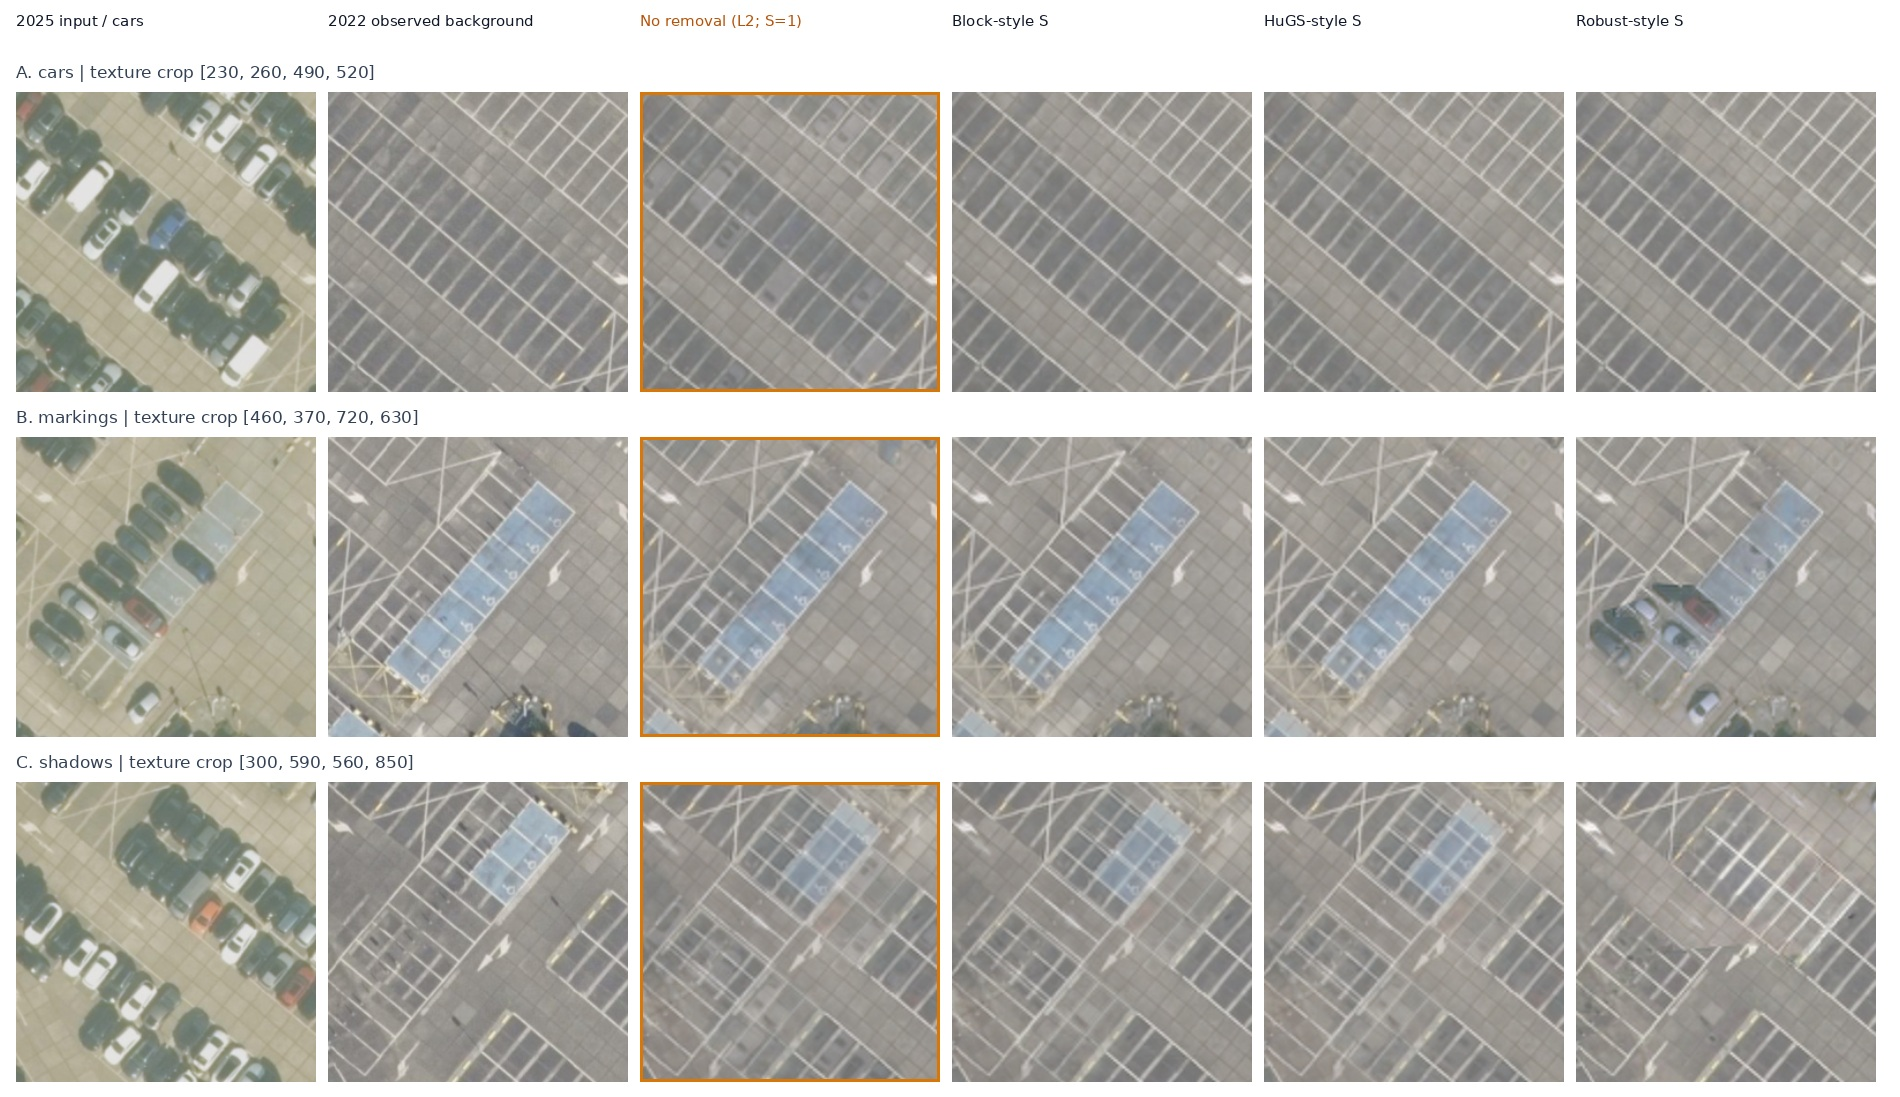
\includegraphics[width=\linewidth,height=.58\textheight,keepaspectratio]{assets/easy_crops.jpg}
\caption{Easy의 미적용 L2 포함 동일 위치 비교. 차량, 주차선, 명암 영역을 함께 보아 표본 점수와 넓은 지면 품질의 차이를 확인한다. 원 저장 결과에서 가져온 그림이며 추가 학습은 하지 않았다.}\end{figure}

\clearpage
\subsection{Hard: 높은 차량 점유에서의 기존 기준선}
\begin{table}[htbp]\centering\small
\caption{Hard의 기존 주요 기준선. 평균$\pm$표본표준편차,3seed. 각 열은 PSNR(dB). B/C의3--4회 점유 OBB는 각각4/17개다.}
\begin{tabular}{llrrr}\toprule 장면 & 방법 & 3--4회 점유 OBB & 관측 가능한 hard 픽셀 & 정적 대조\\\midrule
B & L2 (no-removal) & 19.01 $\pm$ 0.18 & 18.94 $\pm$ 0.17 & 21.97 $\pm$ 0.37 \\
B & Block-type & 19.94 $\pm$ 0.21 & 19.85 $\pm$ 0.20 & 21.85 $\pm$ 0.29 \\
B & HuGS-type & 18.16 $\pm$ 0.10 & 18.03 $\pm$ 0.10 & 21.01 $\pm$ 0.34 \\
B & Robust (base) & 14.49 $\pm$ 0.36 & 14.37 $\pm$ 0.37 & 19.71 $\pm$ 0.21 \\
C & L2 (no-removal) & 18.69 $\pm$ 0.24 & 19.17 $\pm$ 0.04 & 24.40 $\pm$ 0.35 \\
C & Block-type & 20.98 $\pm$ 0.19 & 22.24 $\pm$ 0.09 & 24.80 $\pm$ 0.09 \\
C & HuGS-type & 20.89 $\pm$ 0.09 & 21.67 $\pm$ 0.10 & 24.33 $\pm$ 0.13 \\
C & Robust (base) & 16.00 $\pm$ 0.40 & 16.80 $\pm$ 0.45 & 23.83 $\pm$ 0.08 \\\bottomrule\end{tabular}\end{table}

기존 주요4방법 중 Block형이 두 장면의 주평가 PSNR에서 가장 높았지만 차량 전체가 사라지지는 않았다. Robust형은 다수 시기에 반복되는 차량을 inlier로 받아들이고 드문 배경을 제외할 수 있다. 시간 중앙값 역시 차량이 다수인 위치에서는 차체 RGB를 선택할 수 있다. 그림자와 미관측 지면도 클래스 마스크만으로 해결되지 않는다.
\begin{table}[htbp]\centering\small
\caption{Hard의 추가 변형(seed42). PSNR은3--4회 점유 OBB, LPIPS는전체 채택 OBB crop 평균이다. 주요 표의3seed 평균과 구분한다.}
\begin{tabular}{lrrrr}\toprule & \multicolumn{2}{c}{B} & \multicolumn{2}{c}{C}\\ 방법 & PSNR & LPIPS & PSNR & LPIPS\\\midrule
L2 (no-removal) & 18.93 & 0.147 & 18.87 & 0.335 \\
Temporal median & 18.48 & 0.119 & 18.85 & 0.338 \\
Block-type & 19.70 & 0.135 & 21.17 & 0.162 \\
HuGS-type & 18.12 & 0.129 & 20.97 & 0.174 \\
Robust (base) & 14.69 & 0.176 & 16.09 & 0.334 \\
Robust (OR) & 14.59 & 0.179 & 16.32 & 0.329 \\
Robust (car) & 14.04 & 0.189 & 18.38 & 0.277 \\
Robust (depth) & 14.23 & 0.175 & 16.74 & 0.299 \\\bottomrule\end{tabular}\end{table}

\begin{figure}[htbp]\centering
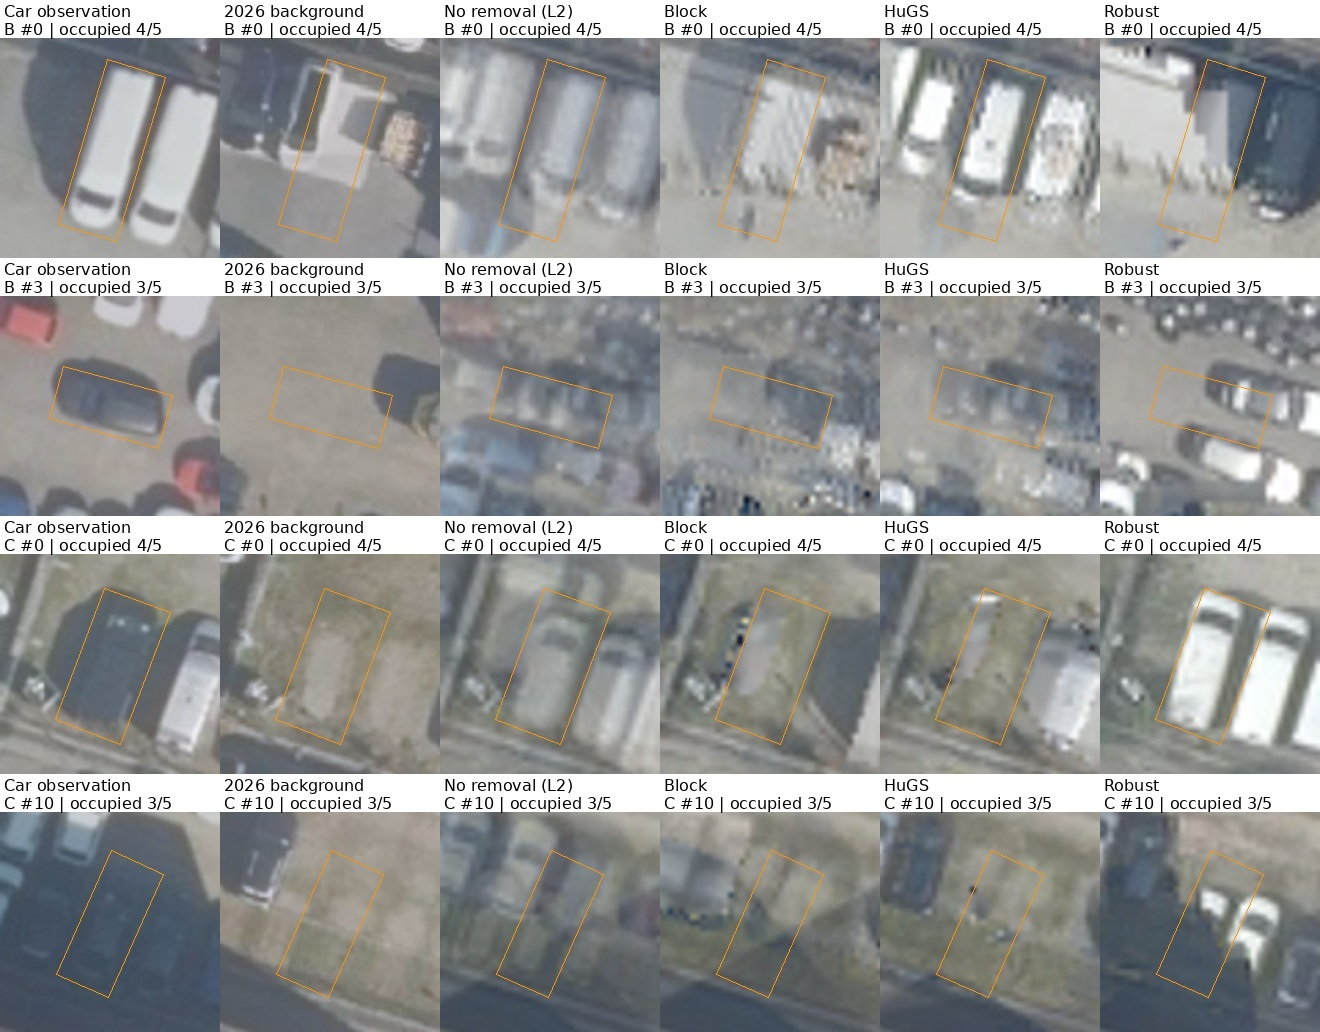
\includegraphics[width=\linewidth]{assets/hard_hero.jpg}
\caption{Hard의 고정 위치 비교. 왼쪽부터 차량 학습 관측,2026 배경, L2, Block형, HuGS형, Robust형이다. B와C에서 각각4/5 및3/5 점유 표본을 사용하며 Improved와 같은 위치다. 주황선은 고정 평가 OBB다.}\end{figure}

\clearpage
\subsection{Improved: 배경 관측 선택과 명시적 공간 prior}
\begin{table}[htbp]\centering\scriptsize
\caption{동일 Hard 평가에서의 개선안. 학습형 PSNR은3seed 평균$\pm$표본표준편차, 다른 열은 평균. UV 직접 합성 두 방법은 결정적 계산1회로 표준편차가 없다.}
\begin{tabular}{lrrrr}\toprule 방법 & B 차량 PSNR & C 차량 PSNR & B / C LPIPS & B / C 정적 PSNR\\\midrule
L2 (no-removal) & 19.01 $\pm$ 0.18 & 18.69 $\pm$ 0.24 & 0.149 / 0.338 & 21.97 / 24.40 \\
Block-type & 19.94 $\pm$ 0.21 & 20.98 $\pm$ 0.19 & 0.136 / 0.165 & 21.85 / 24.80 \\
HuGS-type & 18.16 $\pm$ 0.10 & 20.89 $\pm$ 0.09 & 0.127 / 0.176 & 21.01 / 24.33 \\
Robust (base) & 14.49 $\pm$ 0.36 & 16.00 $\pm$ 0.40 & 0.173 / 0.342 & 19.71 / 23.83 \\
UV fusion & 20.81 & 22.10 & 0.085 / 0.146 & 24.51 / 26.62 \\
UV + shadow guard & 21.00 & 22.23 & 0.079 / 0.130 & 24.58 / 26.47 \\
Geometry mask & 19.95 $\pm$ 0.15 & 20.86 $\pm$ 0.09 & 0.118 / 0.183 & 21.68 / 24.89 \\
Geometry + init & 19.94 $\pm$ 0.17 & 21.33 $\pm$ 0.10 & 0.118 / 0.178 & 21.68 / 24.90 \\
Geometry + prior & 20.39 $\pm$ 0.23 & 21.74 $\pm$ 0.11 & 0.114 / 0.170 & 21.83 / 25.08 \\\bottomrule\end{tabular}\end{table}

그림자 guard를 추가한 UV fusion은 Block형에 비해 B 약1.06dB, C 약1.25dB 높았다. LPIPS도 낮아졌다. 다만 guard 없는 UV fusion과 비교하면 C 정적 대조 PSNR은26.62에서26.47dB로 소폭 감소해, 모든 지표에서 일관된 개선은 아니다.

Geometry mask만으로는 개선이 작았고, fusion 초기화의 이득도600회 최적화 후 일부 사라졌다. 공간 prior는 Geometry + init 대비 주평가 PSNR을 B 약0.45dB, C 약0.41dB 높였지만 직접 fusion보다 낮았다. 알려진 평면 UV에서는 직접 관측 합성이 역렌더링 최적화보다 유리한 실용 기준선이었다. 이 비교는 원래 NeRF 환경에서의 우열을 뜻하지 않는다.

\begin{figure}[htbp]\centering
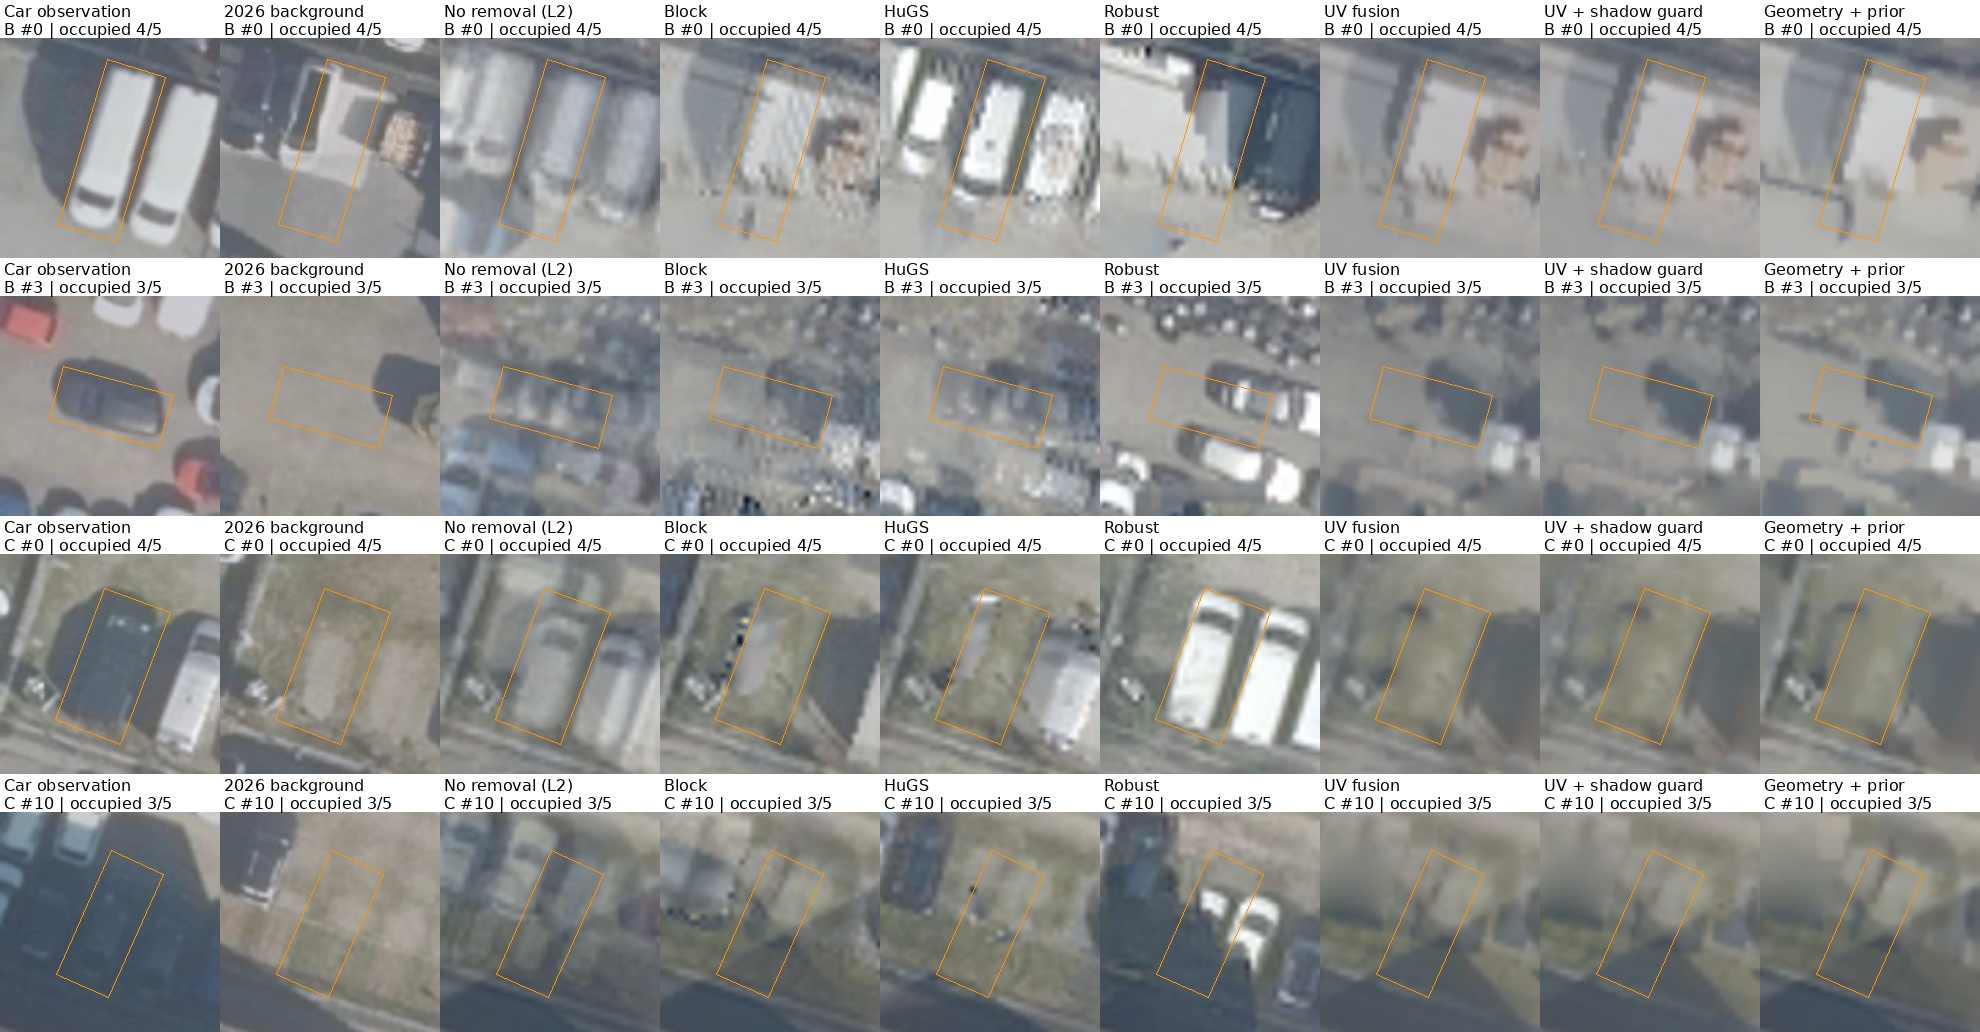
\includegraphics[width=\linewidth]{assets/improved_crops.jpg}
\caption{동일4개 고정 차량 위치의 개선안 비교. 주황선은 평가 OBB로 시각화에만 표시했다. 모든 결과는seed42, 동일 cropㆍ동일 색 범위다. UV 합성에서 차체와 중첩 흔적은 줄지만 일부 어두운 흔적과 주변 차량은 남는다. 폴리곤 밖 인접 차량은 해당 표본 점수에 포함되지 않는다.}\end{figure}

\begin{figure}[p]\centering
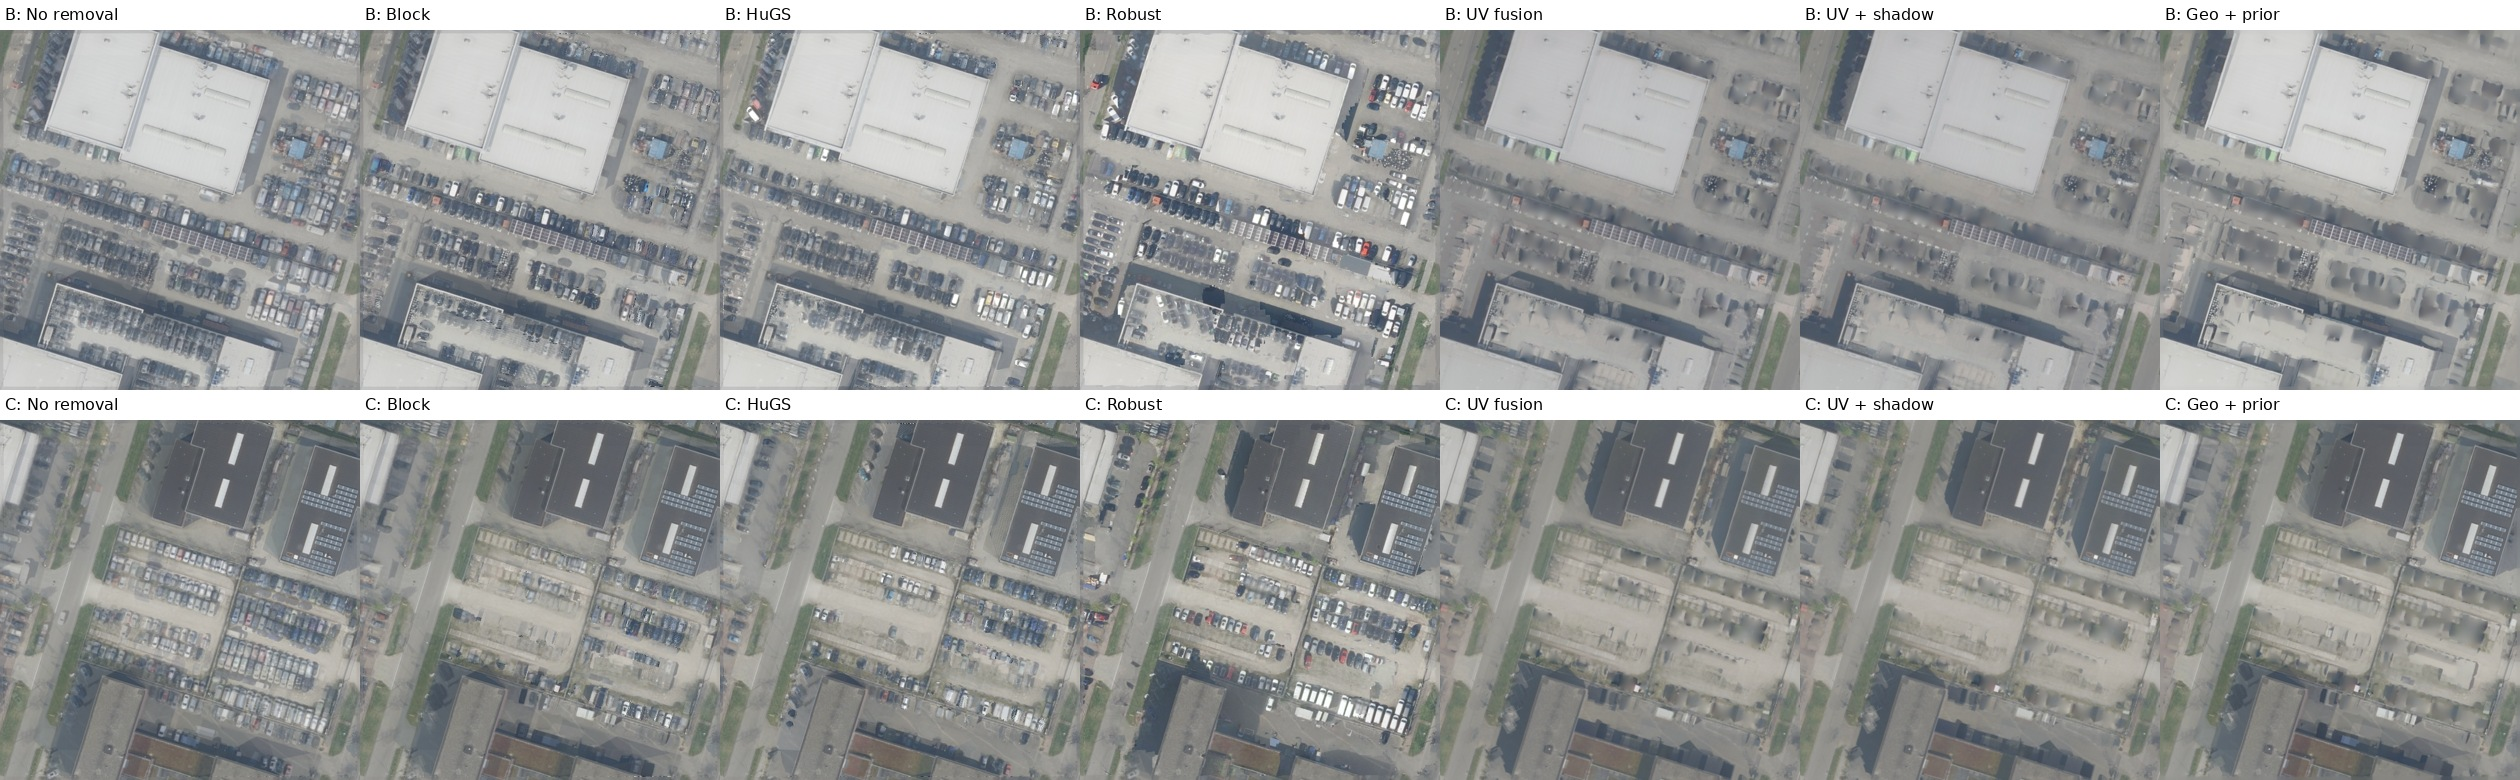
\includegraphics[width=\linewidth]{assets/improved_full.jpg}
\caption{전체 장면 비교. 윗줄B, 아랫줄C. 미적용 L2, Block형, HuGS형, Robust형, UV fusion, UV+shadow guard, Geometry+prior 순서다. 미관측 영역의 보간ㆍ그림자ㆍ주변 잔류 차량까지 포함해 보아야 한다.}\end{figure}

\subsection{해석, 한계 및 재현 범위}
\begin{enumerate}
\item \textbf{관측 선택의 효과:} 잔차가 작다는 사실과 정적 배경이라는 사실은 다르다. 의미 마스크로 차량 관측을 제외하면 소수 배경도 사용할 수 있지만 검출 누락은 그대로 영향을 준다.
\item \textbf{복원과 보간의 구별:} 5회 모두 가린 영역은 색을 직접 관측하지 못했다. 조화 보간ㆍTVㆍanchor는 공간적 추정으로, 실제 배경의 정확한 복원을 입증하지 않는다. 차선과 작은 디테일 손실도 남는다.
\item \textbf{공정성의 범위:} 학습형은 동일600회ㆍ동일 Adam 설정이지만 HuGS는 추가 warm-up/SIFT/SAM 비용이 있다. 직접 fusion은 최적화가 없고 학습형 affine 색보정도 없으므로 계산 비용ㆍ모델군까지 같지는 않다. 원 중앙값 참고 기준선은512기저도 거치지 않았다.
\item \textbf{통계와 평가:} 3seed의 표준편차는 동일 장면의 최적화 변동이며 독립3장면이나 신뢰구간이 아니다. Hard 주평가는 B4개, C17개로 작고 불균형하다. detector 기반 위치ㆍ점유와 실제2026년의 조명ㆍ토양ㆍ계절 변화에 따른 편향이 남는다.
\item \textbf{설계와 일반화:} Improved는 같은 benchmark의 이전 실패를 보고 설계했다.2026 RGB나 annotation을 fusionㆍ최적화에 쓰지는 않았지만 외부 미관측 데이터 검증으로 해석할 수 없다. 반합성 카메라는 실제 사선 촬영의3D parallax가 없고, 두 Hard 장면도 같은 산업지구다.
\end{enumerate}

현재 조건의 실용적 기준선은 비차량 UV fusion이며, 어두운 흔적을 줄이려면 고정 shadow guard를 함께 비교할 수 있다. 전체 차량 제거의 보증이 아닌 개선된 출발점이다. 본 통합 문서는 저장된 실험을 재정리한 것이며 새 학습이나 평가 영역 변경은 수행하지 않았다.

\subsection{산출물과 실행 기록}
원 프로젝트 기준 주요 파일은 다음과 같다.
\begin{itemize}
\item Easy: \path{PROJECT_EASY_PILOT.md}, \path{pilot.py}, \path{results/metrics.csv}, \path{results/manual_metrics.csv}.
\item Hard: \path{PROJECT_HARD_BASELINES.md}, \path{harder_dataset/run_scene.py}, \path{harder_dataset/evaluate_harder.py}, \path{harder_dataset/results/metrics.csv}.
\item Improved: \path{PROJECT.md}, \path{harder_dataset/improved_baselines/train.py}, \path{shadow_guard.py}, \path{protocol.json}, \path{shadow_protocol.json} (마지막3개도 같은 improved 디렉터리).
\item 통합 지표: \path{harder_dataset/improved_baselines/results/combined_metrics.csv}.54행은 기존32행과 신규22행이다. 신규는18개600회 학습 실행과4개 결정적fusion이다.
\item 신규 검증: \path{harder_dataset/improved_baselines/results/validation.json}. 관측 median 보존, 마스크ㆍ수치 유효성, 반복 예산, 기존 L2 점수 동일 재계산을 확인했다.
\item 이 LaTeX 폴더의 \path{source_manifest.json}에 통합에 사용한 문서ㆍ코드ㆍ지표의 체크섬을 남겼다. 표는 저장된 CSV에서 생성했으며 새 수치를 추정하지 않았다.
\end{itemize}

\begin{thebibliography}{9}
\bibitem{pdok} PDOK / Beeldmateriaal Nederland. Luchtfoto RGB open. \url{https://www.pdok.nl/introductie/-/article/pdok-luchtfoto-rgb-open-}. 출처ㆍ라이선스 안내: \url{https://www.beeldmateriaal.nl/dataroom}.
\bibitem{block} Tancik et al. Block-NeRF: Scalable Large Scene Neural View Synthesis. CVPR, 2022. 본 실험은 의미 클래스 마스킹 아이디어를 차용하고 항공 OBB 검출기로 대체했다.
\bibitem{hugs} NeRF-HuGS, 공식 구현. \url{https://github.com/cnhaox/NeRF-HuGS}. 마스크 생성 코드: \path{HuGS/generate_static_mask.py}. 본문 수식은 본 실험의 실제 대체 구현을 기술한다.
\bibitem{robust} Sabour et al. RobustNeRF: Ignoring Distractors with Robust Losses. CVPR, 2023. 공식 MultiNeRF 코드: \url{https://github.com/google-research/multinerf/blob/main/internal/robustnerf.py}.
\bibitem{sam} Kirillov et al. Segment Anything. ICCV, 2023. \url{https://github.com/facebookresearch/segment-anything}.
\bibitem{obb} Ultralytics OBB documentation. \url{https://docs.ultralytics.com/tasks/obb/}. 본 파일럿은 DOTA 사전학습 YOLO11s-OBB를 사용했다.
\end{thebibliography}
\end{document}
